\chapter{Conclusão}

Uma vez finalizado o projeto, podemos concluir que os objetivos propostos foram alcançados com sucesso. Construímos uma base de conhecimento de acordo com o que era pretendido no enunciado e implementámos as funcionalidades necessárias. Para além disso, decidimos ainda implementar algumas caracteristicas ou funcionalidades que achamos que seriam interessantes incluir neste sistema. Analisando os resultados obtidos, temos que todas as funcionalidades funcionam de acordo com as nossas expetativas e estão de acordo com a nossa base de conhecimento. Um dos problemas com a realização deste exercício está relacionada com a área creativa do grupo, pois tivemos de inventar/imaginar novas funcionalidades úteis para integrar neste exercício, algo que teve de ser bastante discutido no grupo. Em suma, estamos muito satisfeitos com o trabalho que desenvolvemos. 

\begin{figure}[<+h+>]
	\centering
	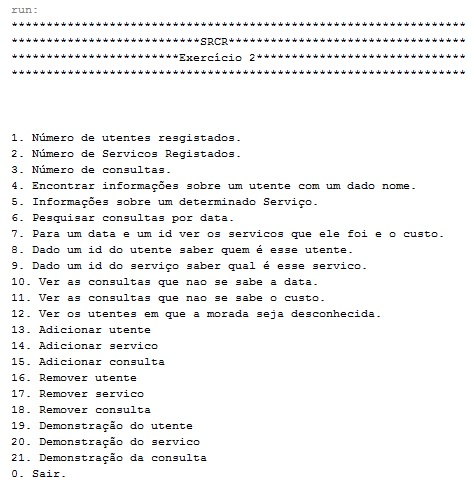
\includegraphics[scale=0.7]{menu.jpg}
	\caption{Menu da aplicação}
\end{figure}